\documentclass[mathserif, xcolor = dvipsnames]{beamer}

\usefonttheme{professionalfonts}
\usecolortheme[named = SeaGreen]{structure}
\usepackage{classico}
\usepackage{mathpazo}
\usepackage[euler-digits]{eulervm}
\usepackage{parskip}

\title{$27$ lines on a cubic}
\author{Jayden Thadani}
\institute{MATH 176 --- Algebraic Geometry}
\date{Fall 2024}

\begin{document}

\frame{\titlepage}

\begin{frame}
	\frametitle{Why should you care?}
	\only<1>{
		No cheats!

		Answers in enumerative geometry often need weasel words like \emph{counted correctly} or \emph{sufficiently general}. There are none here --- the theorem below is exactly true!

		\begin{theorem}
			Every smooth cubic surface in $\overline{k} \mathbb{P}^{3}$ contains exactly $27$ lines.
		\end{theorem}
	}
	\only<2>{
		This is a first example of some really deep algebraic geometry --- enumerative geometry, intersection theory, deformation theory, and so many more!

		Its proofs are an introduction to many powerful tools of algebraic geometry --- parameter and moduli spaces, birational equivalences, and blowups.

		Lie algebras! The $27$ lines obey beautiful symmetries from Lie theory.
	}
	\only<3>{
		Look how pretty!
		\begin{figure}
			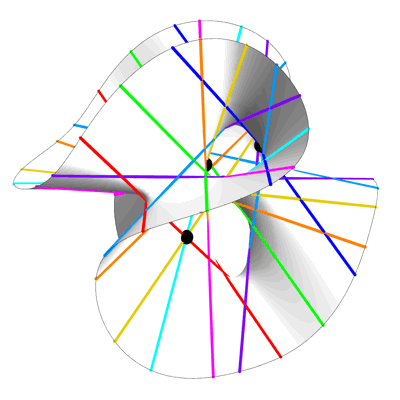
\includegraphics[height = 0.6 \textheight]{figures/27-lines-11.png}
			\caption{The $27$ lines on the Clebsch cubic surface (Greg Egan)}
		\end{figure}
	}
\end{frame}

\end{document}
